\documentclass[12pt]{article} % Sets the base font size (12pt) and document class (article)

% --- Language and Encoding ---
\usepackage[english]{babel} % Sets the language for hyphenation patterns, date formats, etc.

% --- Bibliography ---
\usepackage[backend=biber, style=apa]{biblatex} % Uses biblatex with the biber backend and APA citation style
\addbibresource{resources.bib} % Specifies the bibliography file (must be in the same directory or provide path)

% --- Hyperlinks and PDF Metadata ---
\usepackage{hyperref} % Enables clickable links within the PDF (e.g., ToC, citations, URLs)
\hypersetup{
    hidelinks, % Hides the borders/colors around links
    colorlinks=true, % Colors the link text instead of using borders
    breaklinks=true, % Allows links to break across lines
    urlcolor=black, % Color for URLs
    citecolor=black, % Color for citation links
    linkcolor=black, % Color for internal links (sections, figures)
    bookmarksopen=false, % Whether PDF bookmarks are initially expanded
    pdftitle={Master's Proposal}, % PDF metadata: Title
    pdfauthor={Cagatay Özcan Jagiello Gutt} % PDF metadata: Author
}

% --- Graphics and Page Layout ---
\usepackage{graphicx} % Allows including images (\includegraphics)
\usepackage{geometry} % For customizing page margins and layout
\geometry{a4paper, margin=1in} % Sets paper size to A4 and all margins to 1 inch
\usepackage{float} % Improves control over floating elements like figures and tables

% --- Captions ---
\usepackage{caption} % For customizing captions of figures and tables
\captionsetup{
    justification=justified, % Justifies caption text
    singlelinecheck=false, % Applies justification even to single-line captions
    labelfont=bf, % Makes the caption label (e.g., "Figure 1:") bold
    % textfont=bf, % Makes the caption text bold (currently commented out)
    margin=1.5em, % Sets left/right margin for caption text
    font={stretch=1.0} % Adjusts line spacing within captions (1.0 is normal)
}

% --- Diagrams and Drawing ---
\usepackage{tikz} % Powerful package for creating graphics programmatically
\usetikzlibrary{arrows.meta, shapes.geometric, positioning, decorations.pathreplacing} % Loads useful TikZ libraries

% --- Text Formatting ---
\usepackage{ragged2e} % Provides improved text alignment options (e.g., \RaggedRight)
\usepackage{enumitem} % Provides enhanced control over list environments (enumerate, itemize)
\usepackage{microtype} % Provides structure to the \hboxes

% --- Colors ---
\usepackage{xcolor} % Enables the use of colors
\definecolor{rubblue}{RGB}{0,51,160} % Defines a custom color 'rubblue' (example)
\definecolor{rubgrey}{RGB}{153,153,153} % Defines a custom color 'rubgrey' (example)

% --- Title Page Specific Packages ---
\usepackage{times} % Uses Times New Roman font (often used for title pages or specific styles)
\usepackage{fancyhdr} % For creating custom headers and footers
\usepackage{csquotes} % Provides context-sensitive quotation facilities (e.g., \enquote)
\usepackage{amsmath} % Enhanced math typesetting (American Mathematical Society)
\usepackage{amsfonts} % Provides math fonts (American Mathematical Society)
\usepackage{amssymb} % Provides additional math symbols (American Mathematical Society)
\usepackage{makecell} % Allows line breaks and formatting within table cells
\usepackage{setspace} % For adjusting line spacing (\setstretch, \singlespacing, etc.)

% --- Section Spacing Customization ---
\usepackage{titlesec} % Allows customization of section headings
\titlespacing*{\section}{0pt}{*1.2}{*0.7} % Adjusts spacing around \section: {left}{before}{after} (*N means N times baseline skip)
\titlespacing*{\subsection}{0pt}{*1.2}{*0.7} % Adjusts spacing around \subsection
\titlespacing*{\paragraph}{0pt}{*1}{*0.5} % Adjusts spacing around \paragraph

% --- Glossaries and Acronyms ---
\usepackage[automake, % Automatically runs makeglossaries if needed (requires shell escape enabled)
            acronym, % Enables acronym handling
            toc, % Adds glossaries to the Table of Contents
            shortcuts, % Provides shorthand commands like \acs, \acp
            nomain, % Disables the main glossary type if only acronyms are used
            nonumberlist, % Suppresses page numbers in the glossary list
            nopostdot, % Removes the period after descriptions in the list
            nogroupskip % Removes vertical space between letter groups in the list
           ]{glossaries}

% --- Define Acronyms Here ---
% Format: \newacronym{label}{short_form}{long_form}
% The 'label' is used in the text with \gls{label}, \Gls{label}, \glspl{label}, etc.
\newacronym{ANS}{ANS}{autonomic nervous system}
\newacronym{PFC}{PFC}{prefrontal cortex}
\newacronym{BIS}{BIS}{Behavioural Inhibition System}
\newacronym{BAS}{BAS}{Behavioural Approach System}
\newacronym{HRV}{HRV}{Heart Rate Variability}
\newacronym{ECG}{ECG}{Electrocardiography}
\newacronym{RMSSD}{RMSSD}{Root Mean Square of Successive Differences}
\newacronym{EDA}{EDA}{Electrodermal Activity}
\newacronym{GSR}{GSR}{Galvanic Skin Response}
\newacronym{SCR}{SCR}{Skin Conductance Responses}
\newacronym{SCL}{SCL}{Skin Conductance Level}
\newacronym{PLV}{PLV}{Phase locking value}
\newacronym{EEG}{EEG}{Electroencephalography}
\newacronym{fNIRS}{fNIRS}{Functional Near-Infrared Spectroscopy}
\newacronym{ROI}{ROI}{regions of interest}
\newacronym{SAM}{SAM}{Self-Assessment Manikin}
\newacronym{HbO2}{HbO2}{Oxyhemoglobin}
\newacronym{HbR}{HbR}{Deoxyhemoglobin}
\newacronym{NN intervals}{NN intervals}{Time intervals between consecutive R-peaks}
\newacronym{ICA}{ICA}{Independent Component Analysis}
\newacronym{TDDR}{TDDR}{temporal derivation distribution repair}
\newacronym{DLPFC}{DLPFC}{dorsolateral prefrontal cortex}
\newacronym{VMPFC}{VMPFC}{ventromedial prefrontal cortex}
\newacronym{ANOVA}{ANOVA}{Analysis of Variance}
\newacronym{FAI}{FAI}{frontal asymmetry index}
\newacronym{P wave}{P wave}{arterial depolarization}
\newacronym{QRS complex}{QRS complex}{ventricular depolarization}
\newacronym{T wave}{T wave}{ventricular repolarization}
\newacronym{GLM}{GLM}{General Linear Model}
\newacronym{PANAS}{PANAS}{Positive and Negative Affect Schedule}
\newacronym{WP}{WP}{Work Packages}

\makeglossaries % Processes the defined glossaries and acronyms

% --- Glossary Formatting ---
\renewcommand*{\glsnamefont}[1]{\textbf{\textit{#1}}} % Formats the acronym name in the list (bold italic)

% --- Header/Footer Setup ---
\renewcommand{\headrulewidth}{0.4pt} % Sets the thickness of the header rule line
\renewcommand{\footrulewidth}{0.4pt} % Sets the thickness of the footer rule line
\setlength{\headheight}{14.49998pt} % Sets the height reserved for the header (adjust if fancyhdr warns)
\addtolength{\topmargin}{-2.49998pt} % Adjusts top margin to compensate for header height changes
\setlength{\parindent}{0 cm} % Sets paragraph indentation to zero (paragraphs separated by vertical space)

% --- Custom Colors (Examples) ---
\definecolor{borot}{RGB}{226,0,26} % Example custom color
\definecolor{Grau}{gray}{0.96} % Example custom color (light gray)

% --- Custom Commands (Examples) ---
\newcommand{\mt}[2][Grau]{\colorbox{#1}{#2}} % Example: Highlight text with a background color
\newcommand{\ts}[1]{\textsl{#1}} % Example: Shortcut for slanted text
\newcommand{\q}[1]{\glqq #1\grqq} % Example: Shortcut for German-style quotes (requires csquotes)

% --- Page Style Setup (using fancyhdr - matching proposal) ---
\pagestyle{fancy} % Activates the fancy page style
\fancyhf{} % Clears all existing header and footer fields
\fancyhead[R]{Neural-Autonomic Synchrony and Embodied Integration} % Use proposal title in header
\fancyhead[L]{\nouppercase{\leftmark}} % Sets the current section title (lowercase) in the top left header
\fancyfoot[C]{-\thepage-} % Sets the page number centered in the footer
\fancyfoot[L]{Cagatay Özcan Jagiello Gutt} % Sets author name in the bottom left footer
\fancyfoot[R]{\href{mailto:cagatay.gutt@rub.de}{cagatay.gutt@rub.de}} % Sets clickable email link in footer

% --- End of Preamble ---


\begin{document} % Start of the document content

% --- Front Matter ---
\pagenumbering{Roman} % Use Roman numerals for page numbers in the front matter

% --- Title Page ---
\begin{titlepage}
    % Content for the title page (university logo, title, author, supervisors, date, etc.)
    \begin{center}
        \begin{minipage}{0.2\textwidth}
            
\includegraphics[width=1.5\textwidth]{EV_images/rub.jpg} % Include university logo (adjust path/size)
        \end{minipage}
        \hspace*{\fill}
        \begin{minipage}{0.6\textwidth}
            \hspace*{\fill}\textbf{Ruhr-University Bochum} \\ \hspace*{\fill}\textbf{Faculty of Psychology}
        \end{minipage}

        \vspace{2 cm}
        {\textbf{\large MASTER THESIS PROPOSAL}}

        \vspace{0.2cm}
        Presented to outline the general concept of the master's thesis in the field of social cognition within the Cognitive Science study program at Ruhr-University Bochum

        \vspace{0.5cm}
        by the student

        \vspace{0.5cm}
        Cagatay Özcan Jagiello Gutt\\
        Student Number: 108022246097

        \vspace{0.5cm}
        Submission Date: 24.04.2025\\
        Examination Period: Summer Semester 2025

        \vspace{0.5cm}
        Thesis Title:

        \vspace{0.2cm}
        \textbf{Neural-Autonomic Synchrony and Embodied Integration}

        \vspace{0.2cm}
        Temporal Binding of Frontal-Parietal Networks and Autonomic Responses in Conscious Emotional Processing

        \vspace{0.5cm}
        \begin{minipage}{0.8\textwidth}
            \begin{tabular}{p{0.4\textwidth} p{0.4\textwidth}}
                1st Supervisor: & Dr. Julian Elias Reiser \\
                & Leibniz Research Centre for Working Environment and Human Factors (IfADo) \\
                & at TU Dortmund, Department of Psychology and Neurosciences\\
                \\
                2nd Supervisor: & Prof. Dr. Dirk Scheele \\
                & Research Department of Neuroscience, Institute of Cognitive Neuroscience, \\
                & Faculty of Psychology, Ruhr-University Bochum \\
            \end{tabular}
        \end{minipage}

        \vspace{\fill} % Pushes content to the top/bottom
    \end{center}
\end{titlepage}

\newpage % Start a new page

% --- Table of Contents ---
\tableofcontents % Generates the Table of Contents

\newpage % Start a new page

% --- List of Figures ---
\phantomsection % Ensures hyperref links correctly to this point
\addcontentsline{toc}{section}{List of figures} % Adds "List of Figures" to the ToC
\listoffigures % Generates the List of Figures

\newpage % Start a new page

% --- List of Acronyms ---
% Prints the glossary list defined earlier, specifically for acronyms
\printglossary[style=long3col, % Uses a three-column style for the list
               type=\acronymtype, % Specifies that only acronyms should be printed
               title=List of Acronyms] % Sets the title for this list


\newpage % Start a new page

% --- Main Content ---
\pagenumbering{arabic} % Switch to Arabic numerals for the main body

% --- Introduction Section ---
\section{Introduction}

% Paragraph 1: General background on emotion, brain-body interaction, clinical relevance - Micro Tweak
The human experience is profoundly shaped by emotions, which orchestrate adaptive responses to environmental challenges and opportunities. Not purely mental events, emotions manifest as complex, integrated states involving subjective feelings, cognitive appraisals, behavioral expressions, and significant physiological changes mediated by the central and \gls{ANS} \parencite{barrettHandbookEmotions2016, kreibigAutonomicNervousSystem2010}. Understanding the dynamic interplay between neural processing and autonomic physiology is fundamental to emotion science \parencite{critchleyNeuralMechanismsAutonomic2005}. This brain-body interaction is not merely epiphenomenal; the perception and regulation of bodily states (interoception) actively contribute to emotional feeling and decision-making \parencite{antoniodamasioDescartesErrorEmotion2005}. Furthermore, disruptions in this neuro-autonomic dialogue, such as altered heart rate variability or electrodermal hypo/hyper-reactivity, are increasingly recognized as core features of affective disorders like anxiety and depression, underscoring the clinical relevance of investigating these mechanisms \parencite{thayerHeartRateVariability2009, beauchaineVagalToneDevelopment2001}.\\

% Paragraph 2: Role of PFC, asymmetry models (motivational direction), BIS/BAS - Micro Tweak
Within the brain, the \gls{PFC} is critical for orchestrating emotional responses, integrating sensory information with internal goals and modulating subcortical affective circuits \parencite{fusterPrefrontalCortex2008}. A prominent theoretical framework focuses on hemispheric asymmetry in \gls{PFC} activity. The motivational direction model posits that relatively greater left \gls{PFC} activation supports approach-related motivation and positive affect, while relatively greater right \gls{PFC} activation underlies withdrawal-related motivation and negative affect \parencite{davidsonWhatDoesPrefrontal2004, harmon-jonesAngerFrontalBrain1996}. This asymmetry is not static but dynamically modulated by emotional context and individual predispositions, such as trait approach/avoidance tendencies captured by the \gls{BIS} and \gls{BAS} scales \parencite{carverBehavioralInhibitionBehavioral1994, suttonPrefrontalBrainAsymmetry1997, rodriguesMindMovementFrontal2018}. The effectiveness of emotional induction methods can also influence the observed asymmetry, suggesting that more engaging stimuli may elicit stronger, more differentiated neural responses \parencite{rodriguesMethodsMatterExamination2021}.\\

% --- CHANGE START: Intro Para 3 (HRV/EDA) - Condensed RMSSD/EDA description ---
% Paragraph 3: Autonomic measures (HRV/ECG/RMSSD, EDA/GSR/SCR/SCL) - Micro Tweaks
While the \gls{PFC} orchestrates central processing, the emotional response simultaneously engages the body via the \gls{ANS}, adjusting physiology to meet situational demands. Different physiological signals offer complementary views of autonomic activity. \gls{HRV}, the analysis of beat-to-beat fluctuations in heart rate derived from \gls{ECG}, provides a non-invasive window into \gls{ANS} function \parencite{malikHeartRateVariability1996, berntsonHeartRateVariability1997}. Short-term metrics like \gls{RMSSD} primarily reflect parasympathetic (vagal) control \parencite{malikHeartRateVariability1996, shafferOverviewHeartRate2017}. Higher vagally-mediated \gls{HRV} (indexed by \gls{RMSSD}) generally reflects greater autonomic flexibility and adaptive capacity, linked to effective emotional regulation, while reduced \gls{HRV} is linked to stress, psychopathology, and impaired executive function \parencite{thayerRelationshipAutonomicImbalance2010}. In contrast, sympathetic activity can be captured using \gls{EDA} (\gls{GSR}), which measures changes in skin conductance driven by sympathetically-innervated sweat glands \parencite{dawsonElectrodermalSystem2007, boucseinElectrodermalActivity2012}. Phasic increases (\gls{SCR}) reflect event-related sympathetic bursts, while the tonic \gls{SCL} indicates general arousal \parencite{boucseinElectrodermalActivity2012}. Capturing both parasympathetic (\gls{RMSSD}) and sympathetic (\gls{EDA}) influences allows comprehensive assessment of the body's response during emotion.\\
% --- CHANGE END: Intro Para 3 ---

% Paragraph 4: Emotion perception theories (appraisal vs. direct perception), embodied cognition link - Micro Tweak
The perception of emotion itself is also debated. While traditional appraisal theories emphasize cognitive interpretation as the primary determinant of emotional experience \parencite{schererAppraisalProcessesEmotion2001}, alternative perspectives like the direct perception account suggest a more immediate recognition of emotional significance based on characteristic patterns of features, akin to perceptual object recognition \parencite{newenEmotionRecognitionPattern2015}. This view aligns well with theories of embodied cognition, which posit that cognitive processes, including emotional understanding, are grounded in the body's sensorimotor and physiological states \parencite{niedenthalEmbodimentEmotionConcepts2009}. From this perspective, the coordinated activity between neural circuits (like the \gls{PFC}) and autonomic responses (reflected in \gls{RMSSD} and \gls{EDA}) is not just a correlate but an integral part of the emotional percept and experience \parencite{critchleyNeuralMechanismsAutonomic2005}. Understanding how these systems dynamically couple (synchronize) over time is key to understanding the emergence of subjective feeling states. \\

% Paragraph 5: Need for synchrony measures, introduction to PLV - Micro Tweak
Investigating this embodied perspective, where coordinated brain-body activity is integral to emotion, necessitates analytical approaches capturing the temporal coordination (synchrony) between brain and body signals. Neural-autonomic synchrony reflects the functional coupling between central neural oscillations and peripheral physiological rhythms \parencite{thayerHeartRateVariability2009}. Quantifying this synchrony reveals how effectively these systems interact during emotional challenges. The \gls{PLV} is a robust method for this purpose \parencite{lachauxMeasuringPhaseSynchrony1999}. \gls{PLV} measures the consistency of the phase difference between two time series, irrespective of their amplitudes. A high \gls{PLV} indicates consistent phase alignment, suggesting a stable functional interaction. We will calculate \gls{PLV} between the \gls{EEG} signal from the \gls{PFC} and two different autonomic signals: separately with a continuous \gls{HRV}-derived signal (reflecting parasympathetic influence) and with a continuous \gls{EDA}-derived signal (reflecting sympathetic influence). Compared to coherence measures, which are sensitive to both phase and amplitude, \gls{PLV}'s focus on phase makes it particularly adept at detecting transient, potentially non-linear synchronization patterns characteristic of dynamic biological systems responding to stimuli \parencite{cohenAnalyzingNeuralTime2014, valenzaRevealingRealTimeEmotional2014}. The proposed theoretical integration is depicted in \autoref{fig:neuralmodel}.\\

% Paragraph 6: Study aims, multimodal approach justification, stimuli, specific measures (EEG bands, autonomic signals) - Micro Tweak
The present study aims to elucidate neural-autonomic synchrony during the conscious processing of distinct emotional states elicited by validated affective stimuli. We adopt a multimodal approach, integrating high-temporal-resolution \gls{EEG} to capture rapid prefrontal neural dynamics, \gls{ECG} to derive measures of primarily parasympathetic autonomic control (\gls{RMSSD}), \gls{EDA} to reflect sympathetic sudomotor control, and \gls{fNIRS} for complementary spatial localization \parencite{scholkmannReviewContinuousWave2014, pintiCurrentStatusIssues2019}. This combination allows investigating network dynamics while focusing on \gls{EEG}'s temporal resolution for synchrony, \gls{ECG}/\gls{EDA} for specific autonomic branches, and \gls{fNIRS} to localize activity in key prefrontal (emotion regulation) and parietal (attention, bodily signal integration) regions \parencite{pessoaRelationshipEmotionCognition2008, critchleyNeuralMechanismsAutonomic2005}. While technically demanding, this integrated approach is necessary to investigate how precisely timed brain-body coupling relates to activity within specific neural substrates. We acknowledge that linking the hemodynamic response measured by \gls{fNIRS} to the specific neural activity whose phase is relevant for autonomic coupling relies on the assumption that significant hemodynamic changes reflect underlying neural engagement relevant to the synchrony analysis, despite the complex and indirect nature of neurovascular coupling \parencite{logothetisInterpretingBOLDSignal2004}. The \gls{fNIRS} data, therefore, serve not just as post-hoc context, but as a means to spatially constrain and interpret the functional significance of observed \gls{EEG}-based synchrony patterns, as detailed in the analysis plan. We will utilize standardized, emotionally evocative video clips (positive, negative, neutral) from the E-MOVIE database, validated by \textcite{maffeiEMOVIEExperimentalMOVies2019} for their efficacy in inducing targeted affective states. By calculating \gls{PLV} between prefrontal \gls{EEG} oscillations (specifically in the alpha [8-13 Hz] and beta [13-30 Hz] bands, which are broadly implicated in cortical processing, attention, and potentially emotional regulation \parencite{klimeschEEGAlphaTheta1999, koenigMillisecondMillisecondYear2002, allenIssuesAssumptionsRoad2004}) and relevant autonomic signals (including continuous signals derived from \gls{HRV} data reflecting vagal activity for brain-heart coupling and continuous phasic \gls{EDA}-derived signals for brain-sudomotor sympathetic coupling), we will investigate how brain-body interactions involving both \gls{ANS} branches vary with emotional content and intensity.\\

% --- Figure Environment for Conceptual Model ---
\begin{figure}[htbp] % h=here, t=top, b=bottom, p=page of floats; ! forces placement
    \centering % Centers the figure content
    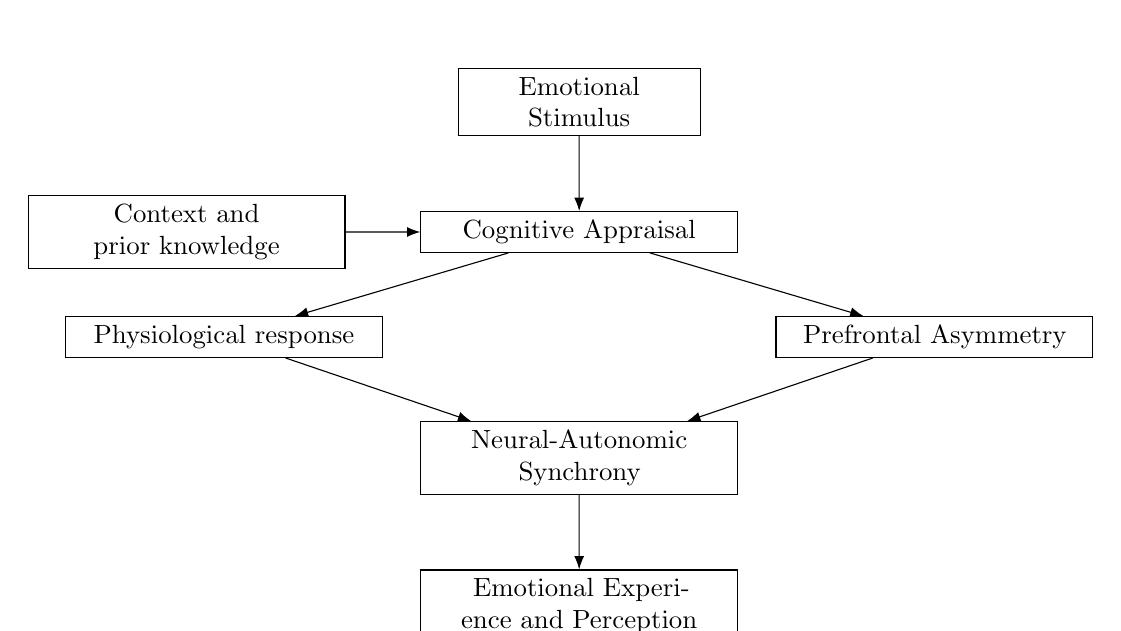
\begin{tikzpicture}[ % Starts the TikZ drawing environment
        scale=0.95, transform shape, % Scales the drawing slightly
        node distance=1cm, % Default distance between nodes
        every node/.style={text width=3cm, align=center}, % Default style for all nodes
        mynode/.style={rectangle, draw}, % Custom style for rectangular nodes with border
        myarrow/.style={-Latex} % Custom style for arrows
    ]
    % --- TikZ Nodes (positioning and content) ---
    \node (A) [mynode] at (0,0) {Emotional Stimulus};
    \node (B) [mynode, below=of A, text width=4cm] {Cognitive Appraisal};
    \node (C) [mynode, left=of B, text width=4cm] {Context and prior knowledge};
    \node (D) [below=of B]{}; % Invisible node for positioning help
    \node (E) [mynode, right=of D, text width=4cm] {Prefrontal Asymmetry};
    \node (F) [mynode, left=of D, text width=4cm] {Physiological response};
    \node (G) [mynode, below=of D, text width=4cm] {Neural-Autonomic Synchrony};
    \node (H) [mynode, below=of G, text width=4cm] {Emotional Experience and Perception};
    % --- TikZ Connections (drawing arrows between nodes) ---
    \draw[myarrow] (A) -- (B);
    \draw[myarrow] (C) -- (B);
    \draw[myarrow] (B) -- (E);
    \draw[myarrow] (B) -- (F);
    \draw[myarrow] (E) -- (G);
    \draw[myarrow] (F) -- (G);
    \draw[myarrow] (G) -- (H);
    \end{tikzpicture}
    \caption{Neural-Autonomic Synchrony in Emotional Experience.} % Figure caption
    \label{fig:neuralmodel} % Label for referencing the figure (\autoref{fig:neuralmodel})
    % \vspace{0.5em} % Optional vertical space after figure
    \parbox{0.8\textwidth}{\scriptsize This diagram illustrates the proposed model of emotional processing, highlighting the interplay between neural and physiological components. An emotional stimulus initiates cognitive appraisal, influenced by contextual factors. Simultaneously, the stimulus elicits a physiological response. Cognitive appraisal leads to prefrontal asymmetry, a key neural component, which interacts with the physiological response through neural-autonomic synchrony. This synchronized activity culminates in the emotional experience.} % Detailed description below caption
\end{figure}

% --- Hypotheses ---
Based on these considerations, we propose the following hypotheses, organized into distinct \gls{WP}:

\begin{enumerate}[label=(\alph*)] % Enumerate hypotheses with (a), (b), etc.
    \item \textbf{Neural-Autonomic Synchrony will be significantly enhanced during the processing of emotional stimuli.} We hypothesize that neural-autonomic synchrony (\gls{PLV}) will be significantly enhanced during the processing of both positive and negative emotional stimuli compared to neutral stimuli. We will investigate this in \gls{WP}1: \emph{Emotional Modulation of Synchrony}, using \gls{PLV} calculated between prefrontal \gls{EEG} and both continuous \gls{HRV}-derived signals (reflecting brain-heart parasympathetic coupling) and \gls{EDA}-derived signals (reflecting brain-sudomotor sympathetic coupling). Rationale: Emotional engagement necessitates greater integration between central command centers and peripheral effectors (cardiac and sudomotor) to prepare for potential action and adapt internal milieu; this heightened integration is expected to manifest as stronger phase coupling involving both \gls{ANS} branches \parencite{critchleyNeuralMechanismsAutonomic2005}. While we predict overall enhancement, we will also exploratorily examine whether the nature or dominant branch of synchrony (e.g., \gls{EEG}-\gls{HRV} vs. \gls{EEG}-\gls{EDA}) differs between positive and negative valence conditions.
    \item \textbf{The magnitude of neural-autonomic synchrony is positively correlated with subjective ratings of emotional arousal.} We hypothesize a positive correlation between the magnitude of neural-autonomic synchrony and subjective ratings of emotional arousal (via the \gls{SAM}) specifically during the positive and negative conditions. This correlation will be tested in \gls{WP}2: \emph{Synchrony and Subject Arousal} for both \gls{PLV} using continuous \gls{HRV}-derived signals (parasympathetic coupling) and \gls{PLV} using \gls{EDA}-derived signals (sympathetic coupling). Rationale: Higher subjective arousal reflects a more intense emotional state, likely involving stronger reciprocal signaling and tighter coupling between the brain's assessment and the body's physiological mobilization. This mobilization involves coordinated adjustments in cardiovascular and sudomotor control (potentially reflected in \gls{EEG}-\gls{HRV} or \gls{EEG}-\gls{EDA} synchrony), leading to more consistent phase relationships between central and peripheral systems \parencite{valenzaRevealingRealTimeEmotional2014, boucseinElectrodermalActivity2012}.
    \item \textbf{Individual differences in baseline parasympathetic regulation is positively assiciated with the degree of neural-autonomic synchrony.} We hypothesize that individual differences in baseline parasympathetic regulation, indexed by resting-state \gls{RMSSD}, will be positively associated with the degree of neural-autonomic synchrony exhibited during the processing of negative emotional stimuli. In \gls{WP}3: \emph{Baseline Vagal Tone and Task-Related Synchrony} PLV will be calculated specifically between \gls{EEG} and continuous \gls{HRV}-derived signals. Rationale: Individuals with higher baseline \gls{RMSSD}, indicative of greater vagal regulatory capacity \parencite{thayerRelationshipAutonomicImbalance2010, shafferOverviewHeartRate2017}, may be better equipped to dynamically coordinate neural and cardiac activity when facing demanding or threatening situations, resulting in more robust task-related brain-heart phase synchrony.
    \item \textbf{The direction of prefrontal cortical asymmetry is differentially associated with the strength of phase synchrony.} We hypothesize that the direction of prefrontal cortical asymmetry, indexed by alpha band [8-13 Hz] power differences (e.g., F3 vs. F4), may be differentially associated with the strength of phase synchrony involving distinct autonomic branches. Specifically, we will exploratorily investigate in \gls{WP}4: \emph{Frontal Asymmetry and Branch-Specific Synchrony}, whether greater relative right \gls{PFC} activation (associated with withdrawal/inhibition) correlates with stronger \gls{EEG}-\gls{HRV} \gls{PLV} (parasympathetic coupling), and whether greater relative left \gls{PFC} activation (associated with approach/action) correlates with stronger \gls{EEG}-\gls{EDA} \gls{PLV} (sympathetic coupling), particularly during emotional conditions. Rationale: This hypothesis explores whether the functional specialization suggested by the motivational direction model \parencite{davidsonWhatDoesPrefrontal2004, harmon-jonesAngerFrontalBrain1996}, typically assessed via power measures, extends to the domain of phase coupling with the autonomic branch potentially most relevant to that motivational state. We acknowledge this is an exploratory step, bridging asymmetry (power) and synchrony (phase) concepts, aimed at generating hypotheses about potential underlying mechanisms linking cortical motivational states to specific patterns of brain-body interaction.
\end{enumerate}

% --- Methods Section ---
\newpage
\section{Methods}

% --- Subsection for each modality/aspect ---
\subsection{Electroencephalography} % Micro Tweak
\gls{EEG} measures electrical brain activity via scalp electrodes, capturing voltage fluctuations from synchronized postsynaptic potentials primarily in cortical pyramidal neurons \parencite{sharmaEmergingTrendsEEG2024, chaddadElectroencephalographySignalProcessing2023}. Its excellent temporal resolution (milliseconds) is crucial for capturing the rapid neural dynamics necessary for phase synchrony analysis (\gls{PLV}) with physiological signals \parencite{cohenAnalyzingNeuralTime2014}. While spatial resolution is limited by volume conduction, \gls{EEG} allows tracking oscillatory activity in specific frequency bands linked to cognitive and affective states. In this study, we focus on the Alpha (8-13 Hz) band, often associated with cortical inhibition, attentional processes, and emotional valence processing (particularly in frontal asymmetry contexts \parencite{allenIssuesAssumptionsRoad2004, allenIssuesAssumptionsRoad2004}), and the Beta (13-30 Hz) band, implicated in sensorimotor processing, maintaining the current cognitive set, and potentially arousal states \parencite{klimeschEEGAlphaTheta1999, engelDynamicPredictionsOscillations2001}. \gls{EEG} will thus provide the primary high-resolution neural signal for assessing frontal asymmetry (via alpha power) and calculating \gls{PLV} (using phase information from both alpha and beta bands).

\subsection{Functional Near-Infrared Spectroscopy} % Micro Tweak
\gls{fNIRS} measures cerebral hemodynamic changes (\gls{HbO2}, \gls{HbR}) linked to neural activity using near-infrared light \parencite{scholkmannReviewContinuousWave2014, jobsisNoninvasiveInfraredMonitoring1977, obrigVisibleImagingHuman2003}. This linkage, known as neurovascular coupling, reflects the increased metabolic demand and subsequent blood flow changes in active brain regions. Offering spatial information complementary to \gls{EEG} \parencite{pintiCurrentStatusIssues2019}, \gls{fNIRS} allows localizing hemodynamic correlates of neural activity within specific cortical regions. In this study, it will be used to identify prefrontal \gls{ROI} showing significant task-related activation, which will then inform the analysis of \gls{EEG}-autonomic synchrony originating from those functionally defined areas.

\subsection{Electrocardiography and Heart Rate Variability} % Micro Tweak
\gls{ECG} records the heart's electrical activity, allowing derivation of \gls{HRV} by analyzing beat-to-beat variations (\gls{NN intervals}), which reflect \gls{ANS} modulation of heart rate \parencite{malikHeartRateVariability1996, berntsonHeartRateVariability1997}. We will focus on the time-domain metric \gls{RMSSD}, calculated as:
% --- Equation Environment for RMSSD ---
\begin{equation} % Math environment for displayed equations
    \text{\gls{RMSSD}} = \sqrt{\frac{1}{N-1} \sum_{i=1}^{N-1} (NN_{i+1} - NN_i)^2}
    \label{eq:rmssd} % Label for referencing the equation (\autoref{eq:rmssd})
\end{equation}
where $NN_i$ is the $i$-th interval and $N$ is the number of intervals. \gls{RMSSD} is sensitive to rapid, high-frequency fluctuations in heart rate and primarily reflects parasympathetic (vagal) influence on the heart \parencite{malikHeartRateVariability1996, shafferOverviewHeartRate2017}. Higher resting \gls{RMSSD} generally indicates greater vagal tone and autonomic flexibility \parencite{thayerRelationshipAutonomicImbalance2010}. For the synchrony analysis, a continuous signal representing vagal influence will be derived from the \gls{NN intervals} (e.g., via interpolation) to compute \gls{PLV} with \gls{EEG} signals.

% --- CHANGE START: Methods 2.4 (EDA) - Condensed sweat gland detail ---
\subsection{Electrodermal Activity} % Micro Tweak
\gls{EDA} (\gls{GSR}) measures skin conductance changes reflecting sympathetic output from eccrine sweat glands (involved in thermoregulation and emotional sweating, solely innervated by the sympathetic nervous system) \parencite{dawsonElectrodermalSystem2007, boucseinElectrodermalActivity2012}. It indicates arousal and sympathetic activation \parencite{kreibigAutonomicNervousSystem2010}. \gls{EDA} is typically measured via skin surface electrodes \parencite{boucseinElectrodermalActivity2012}. The signal includes tonic \gls{SCL} (baseline arousal) and phasic \gls{SCR} (event-related bursts) \parencite{dawsonElectrodermalSystem2007}. As we are interested in dynamic coupling related to emotional events, the continuous phasic \gls{EDA} signal will be the focus for \gls{PLV} analysis.
% --- CHANGE END: Methods 2.4 ---

% --- CHANGE START: Methods 2.5 (Setup) - Removed Roy citation ---
\subsection{Experimental Setup} % Micro Tweak
This study employs a multimodal approach, simultaneously recording \gls{fNIRS}, \gls{EEG}, \gls{EDA}, and \gls{ECG}. \gls{fNIRS} (NIRSport, 8 sources/7 detectors, 17 channels + short channels \parencite{gagnonShortSeparationChannel2012}) optodes integrated into an \gls{EEG} cap will cover prefrontal and parietal cortices \parencite{chenStrategicIntegrationCrossDisciplinary2024}. This coverage targets key regions for emotional processing (\gls{PFC} \parencite{fusterPrefrontalCortex2008, etkinEmotionalProcessingAnterior2011}) and parietal areas involved in attention modulation and integrating bodily signals relevant to emotion \parencite{pessoaRelationshipEmotionCognition2008, critchleyNeuralMechanismsAutonomic2005, culhamHumanParietalCortex2006}. While enabling broader network analysis, parietal signals primarily provide context for the focused frontal-autonomic synchrony investigation. Inter-optode distance $\leq$ 3 cm; sampling 7.81 Hz \parencite{scholkmannReviewContinuousWave2014}. \gls{EEG} electrodes (10-20 system with 64 electrodes, excluding optode positions \parencite{sharmaEmergingTrendsEEG2024}) and Polybox-integrated \gls{ECG} (3-lead) / \gls{EDA} (non-dominant hand fingers) modules will record at 1000 Hz \parencite{luckIntroductionEventRelatedPotential2014}. For \gls{EEG} and \gls{fNIRS} electrode placement see \autoref{fig:eegsetup}.
% --- CHANGE END: Methods 2.5 ---

% --- Figure Environment for Setup Diagram ---
\begin{figure}[htbp]
    \centering
    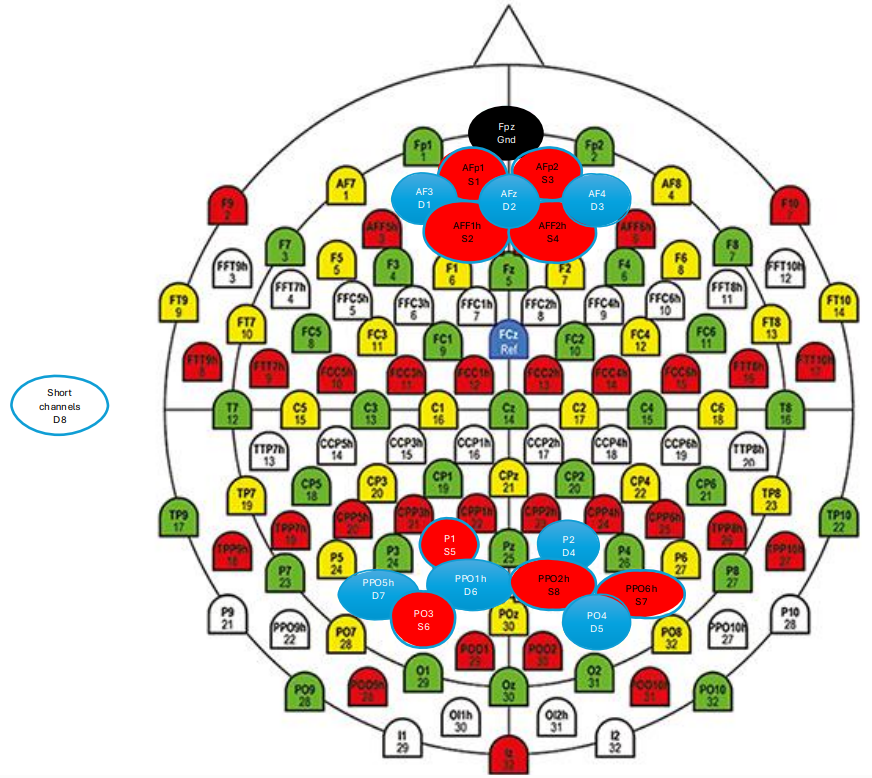
\includegraphics[width=0.48\textwidth]{EV_images/EV_cogMeasSetupMod.png} % Include setup image (adjust path/size)
    \caption{Placement Setup for Simultaneous \gls{EEG} and \gls{fNIRS}.} % Figure caption
    \label{fig:eegsetup} % Label for referencing
    \parbox{0.8\textwidth}{\scriptsize Combined \gls{EEG}/\gls{fNIRS} setup. Blue = detectors, Red = sources. Circled sources connect to short channel detectors.} % Detailed description
\end{figure}

\subsection{Experimental Design} % Micro Tweaks
% Details about stimuli, procedure, randomization, participants
This study utilizes a within-subjects design where participants view emotionally evocative video clips intended to induce positive, negative, or neutral affective states. The stimuli consist of standardized clips selected from the E-MOVIE database \parencite{maffeiEMOVIEExperimentalMOVies2019}, chosen for validated effectiveness and translated to German. To manage presentation and minimize order effects, three bundles are created, each containing one randomly ordered scene of each valence (positive, negative, neutral). Bundle presentation order is counterbalanced across participants, with the constraint that the valence of the last scene in one bundle differs from the first scene of the subsequent bundle. We aim to recruit 20-30 participants for this study.

Before the task, participants complete baseline questionnaires (\gls{BIS}/\gls{BAS} \parencite{carverBehavioralInhibitionBehavioral1994, strobelDeutschsprachigeVersionBIS2006}, \gls{PANAS} \parencite{watsonDevelopmentValidationBrief1988,breyerDeutscheVersionPositive2016}). The experimental procedure involves repeating a specific trial structure nine times (once for each scene). Each trial involves: 1-min baseline rest, video clip presentation, 2-min recovery rest, and post-stimulus questionnaires (\gls{SAM} for valence/arousal, emotional adjectives, basic emotion evaluation, familiarity rating \parencite{maffeiEMOVIEExperimentalMOVies2019}). Breaks and fatigue monitoring are included due to session length.

% REVISED Participant Criteria
Participants (target N=20-30) will be right-handed native German speakers (18-30y), screened for neurological/psychiatric history, current psychopharmaceutical use, scalp conditions impeding sensors, and prior brain stimulation participation.

\subsection{Data Analysis and Statistics} % Micro Tweaks
Data analysis will be conducted using the Python scientific ecosystem \parencite{harrisArrayProgrammingNumPy2020, virtanenSciPy10Fundamental2020}, primarily using MNE-Python \parencite{gramfortMEGEEGData2013} for EEG/MEG, NeuroKit2 \parencite{makowskiNeuroKit2PythonToolbox2021} for physiological signal processing, MNE-NIRS \parencite{yucelBestPracticesFNIRS2021} for fNIRS analysis, and `statsmodels` \parencite{seaboldStatsmodelsEconometricStatistical2010} and `pingouin` \parencite{vallatPingouinStatisticsPython2018} for statistics. The significance level will be set at $p < 0.05$. Standard assumptions (e.g., normality, sphericity) will be checked, using corrections (e.g., Greenhouse-Geisser) or non-parametric tests where appropriate \parencite{fieldDiscoveringStatisticsUsing2024}. Effect sizes will be reported for all key findings. Given the multiple hypotheses and comparisons involved, we will primarily control the False Discovery Rate (FDR) using the Benjamini-Hochberg procedure \parencite{benjaminiControllingFalseDiscovery1995} applied across relevant families of tests (e.g., ANOVA results, correlation analyses).

% --- CHANGE START: Methods 2.7 (Preprocessing) - Removed Roy citation, shortened last sentence ---
\paragraph{Preprocessing and Feature Extraction}
Standard preprocessing pipelines will be applied using the specified Python libraries. \gls{EEG} data will undergo filtering and re-referencing, followed by segmentation relative to stimulus onset. Artifacts (e.g., eye blinks, muscle activity) will be identified and corrected using \gls{ICA} \parencite{delormeEEGLABOpenSource2004}. For \gls{ECG}, data will be filtered, R-peaks detected \parencite{panRealTimeQRSDetection1985}, and \gls{NN intervals} derived to calculate baseline and potentially time-varying \gls{RMSSD} (see \autoref{eq:rmssd}) \parencite{malikHeartRateVariability1996}. \gls{EDA} signals will be filtered and decomposed into tonic (\gls{SCL}) and phasic (\gls{SCR}) components \parencite{benedekDecompositionSkinConductance2010}, with the continuous phasic signal extracted for synchrony analysis \parencite{boucseinElectrodermalActivity2012}. \gls{fNIRS} processing involves converting raw optical density to \gls{HbO2}/\gls{HbR} concentration changes via the modified Beer-Lambert law \parencite{copeSystemLongtermMeasurement1988}, addressing motion artifacts (e.g., using \gls{TDDR} \parencite{scholkmannReviewContinuousWave2014}), filtering (e.g., 0.01-0.1 Hz) to isolate the hemodynamic response, and calculating average concentration changes relative to baseline within predefined prefrontal \gls{ROI}s (e.g., \gls{DLPFC}, \gls{VMPFC} \parencite{etkinEmotionalProcessingAnterior2011, motzkinVentromedialPrefrontalCortex2015}). These \gls{fNIRS} results provide spatial context for the \gls{EEG} synchrony analysis.
% --- CHANGE END: Methods 2.7 (Preprocessing) ---

% --- CHANGE START: Methods 2.7 (Synchrony/Stats) - Shortened PLV description ---
\paragraph{Neural-Autonomic Synchrony and Statistical Testing} % Micro Tweaks
Neural-autonomic synchrony will be quantified using \gls{PLV} \parencite{lachauxMeasuringPhaseSynchrony1999} between prefrontal \gls{EEG} and continuous autonomic signals. \gls{PLV} measures the phase difference consistency ($\Delta\phi(t) = \phi_{\text{EEG}}(t) - \phi_{\text{Autonomic}}(t)$) over a time window:
% --- CHANGE END: Methods 2.7 (Synchrony/Stats) ---
\begin{equation}
    \text{PLV} = \left| \frac{1}{N} \sum_{t=1}^{N} \exp(i \cdot \Delta\phi(t)) \right|
    \label{eq:plv} % Added label for PLV
\end{equation}
where $N$ is the number of time points in the window, $i$ is the imaginary unit, and $\phi_{\text{EEG}}(t)$ and $\phi_{\text{Autonomic}}(t)$ are the instantaneous phases of the filtered \gls{EEG} and the respective continuous autonomic signal (derived from \gls{HRV} or \gls{EDA}) at time $t$. For brain-heart (parasympathetic) coupling, the discrete \gls{NN intervals} will be interpolated into a continuous signal (e.g., using cubic splines at 4 Hz, a standard approach \parencite{lagunaPowerSpectralDensity1998, shafferOverviewHeartRate2017}) via `scipy.interpolate` \parencite{virtanenSciPy10Fundamental2020}. For brain-sudomotor (sympathetic) coupling, the continuous phasic \gls{EDA} signal will be resampled (e.g., to 4 Hz) to match the \gls{HRV}-derived signal's rate. Instantaneous phase will be extracted from filtered \gls{EEG} (Alpha/Beta bands) and continuous autonomic signals via Hilbert transform \parencite{virtanenSciPy10Fundamental2020}. \gls{PLV} (see \autoref{eq:plv}) will then be computed between selected frontal \gls{EEG} channels (e.g., F4/F3, Fp2/Fp1 \parencite{rodriguesMethodsMatterExamination2021}, further refined by \gls{fNIRS} findings as described below) and the continuous \gls{HRV}-derived and phasic \gls{EDA} signals, respectively. The primary analysis window will cover the duration of each stimulus presentation, with comparisons made to \gls{PLV} calculated during the pre-stimulus baseline. Exploratory analyses might examine temporal dynamics within the stimulus period, and surrogate data testing (e.g., phase shuffling \parencite{cohenAnalyzingNeuralTime2014}) may be used to assess significance against chance.

Specific statistical tests will address the hypotheses:
\begin{enumerate}[label=(\alph*)]
    \item \textbf{\gls{WP}1: \emph{Emotional Modulation of Synchrony}.} We will first analyze the \gls{fNIRS} data using a \gls{GLM} approach to identify prefrontal \gls{ROI}s significantly modulated by emotional content (Emotion vs. Neutral contrast) \parencite{yucelBestPracticesFNIRS2021}. \gls{EEG} channels spatially corresponding to these functionally identified ROIs will then be selected \parencite{gramfortMEGEEGData2013}. The primary test for emotional modulation of synchrony will be a repeated measures \gls{ANOVA} on the \gls{PLV} values (\gls{EEG}-\gls{HRV} and \gls{EEG}-\gls{EDA}) from these selected channels, with Emotion (Positive, Negative, Neutral) as the within-subjects factor. Significant effects will be followed by FDR-corrected post-hoc tests. This integrated approach ensures that the synchrony analysis focuses on functionally relevant cortical areas.
    \item \textbf{\gls{WP}2: \emph{Synchrony and Subjective Arousal}.} Pearson correlations will be computed between subjective arousal ratings (\gls{SAM}) and the corresponding trial's \gls{PLV} magnitudes (\gls{EEG}-\gls{HRV} and \gls{EEG}-\gls{EDA} from the functionally defined channels/ROIs), specifically within the positive and negative emotional conditions.
    \item \textbf{\gls{WP}3: \emph{Baseline Vagal Tone and Task-Related Synchrony}.} A Pearson correlation will assess the relationship between resting-state \gls{RMSSD} (baseline parasympathetic tone) and the average \gls{EEG}-\gls{HRV} \gls{PLV} observed during the negative emotional condition (using PLV from the functionally defined channels/ROIs).
    \item \textbf{\gls{WP}4: \emph{Frontal Asymmetry and Branch-Specific Synchrony}.} Frontal asymmetry will be quantified using the \gls{FAI}, calculated from alpha band power differences between homologous frontal electrodes (e.g., F4/F3, Fp2/Fp1 \parencite{rodriguesMethodsMatterExamination2021, allenIssuesAssumptionsRoad2004}). The formula is given by:
    \begin{equation}
        \text{FAI} = \ln(P_{\text{Right}}) - \ln(P_{\text{Left}})
        \label{eq:fai} % Label for FAI equation
    \end{equation}
    where $P_{\text{Right}}$ and $P_{\text{Left}}$ represent the alpha band power spectral density at homologous right and left frontal electrode sites, respectively (e.g., $P_{\text{F4}}$ and $P_{\text{F3}}$). We will then exploratorily test for correlations (Pearson) between this \gls{FAI} and the strength of \gls{EEG}-\gls{HRV} \gls{PLV} versus \gls{EEG}-\gls{EDA} \gls{PLV} (from functionally defined channels/ROIs), particularly during emotional conditions, to investigate potential differential links between cortical motivational direction and coupling with specific autonomic branches.
\end{enumerate}

% --- Timeline Section --- REVERTED TO ORIGINAL BULLET LIST FORMAT
\newpage
\section{Timeline}
% Detailed breakdown of project phases and tasks
\subsection{Phase 1: Preparation (Months 1-2)}
\begin{itemize}
    \item Movie clip acquisition (Month 1)
    \item Writing experiment description (Month 1)
    \item Obtain EEG measurement setup (Month 1)
    \item Obtain fNIRS measurement setup (Month 1)
    \item Participant announcement (Month 1)
    \item Printing new fNIRS Optode holders (Month 1)
    \item Write declaration of consent (Month 1)
    \item Apply for internal email account (Month 1)
    \item Programming task (Month 2)
    \item Ethics approval (Month 2)
    \item Laboratory coordination (Month 2)
    \item Obtain ECG measurement setup (Month 2)
    \item Initial Literature Research (Months 1-2)
\end{itemize}

\subsection{Phase 2: Data Acquisition and Early Analysis, Writing (Months 3-6)}
\begin{itemize}
    \item Piloting (Month 3)
    \item Introducing participants (Month 3)
    \item Ongoing Data Collection (Months 4-6)
    \item On-the-Go Data Preprocessing and Analysis (Months 3-6)
    \item Preliminary Data Analysis (Months 3-6)
    \item Refine Literature Review (Months 3-6)
    \item Drafting Methods Section (Months 3-6)
    \item Drafting Introduction Section (Months 3-6)
    \item Start Drafting Results (Months 5-6)
\end{itemize}

\subsection{Phase 3: Finishing Analysis and Interpretation (Month 7)}
\begin{itemize}
    \item Final Data Preprocessing (Month 7)
    \item Final Data Analysis (Month 7)
    \item Finish Drafting Results (Month 7)
    \item Interpretation of Results (Month 7)
    \item Drafting Discussion Section (Month 7)
\end{itemize}

\subsection{Phase 4: Finalizing and Submission (Months 8-9)}
\begin{itemize}
    \item Refining Introduction Section (First Week of Month 8)
    \item Refining Methods Section (First Week of Month 8)
    \item Refining Results Section (Second Week of Month 8)
    \item Refining Discussion Section (Second Week of Month 8)
    \item Polishing and Proofreading (Third Week of Month 8)
    \item Supervisor Feedback and Revisions (Fourth Week of Month 8)
    \item Final Revisions (First Week of Month 9)
    \item Thesis Submission (Second Week of Month 9)
    \item Buffer (Third and Fourth Week of Month 9)
\end{itemize}

% --- Bibliography Section ---
\newpage % Start bibliography on a new page
\addcontentsline{toc}{section}{References} % Add "References" to the ToC
\printbibliography % Prints the bibliography based on citations in the text and the .bib file

\end{document} % End of the document
